
\documentclass{article}

\usepackage{a4wide,tikz}
\usetikzlibrary{mindmap,trees}
\begin{document}
\pagestyle{empty}


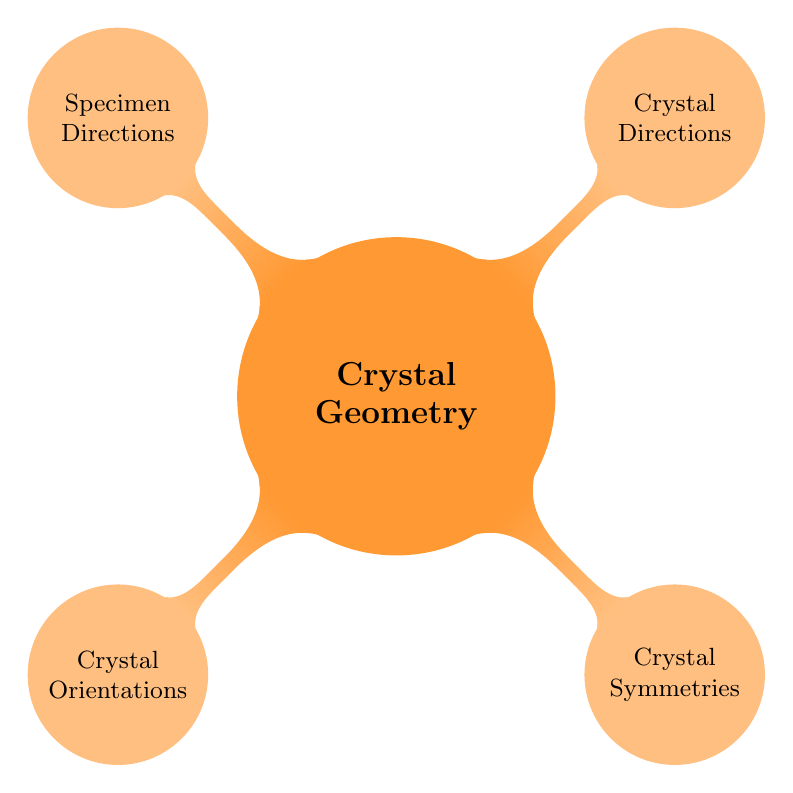
\begin{tikzpicture}[scale = 1]
  \definecolor{myblue}{HTML}{92dcec}
  \tikzstyle{every annotation}=[fill=white, font=\sf]

  \path[mindmap, concept color=orange!80!]
  node[concept] {\bf Crystal\\ Geometry} 
  child[grow = 135, concept color=orange!50] 
  { node(ebsd) [concept](ebsd2) {Specimen Directions}}
  child[grow = 45, concept color=orange!50] 
  { node[concept](pf) {Crystal Directions}}
  child[grow = -135, concept color=orange!50] 
  { node[concept](pf) {Crystal Orientations}}
  child[grow = -45, concept color=orange!50] 
  { node[concept](pf) {Crystal Symmetries}};


\end{tikzpicture}
\end{document}
%%% Local Variables: 
%%% mode: latex
%%% TeX-master: t
%%% End: 
